%%%%%%%%%%%%%%%%%%%%%%%%%%%%%%%%%%%%%%%%%%%%%%%%%%%%%%%%%%%%%%%%%%%%%%%
%% AGI-22 paper about temporal and procedural reasoning with OpenCog %%
%%%%%%%%%%%%%%%%%%%%%%%%%%%%%%%%%%%%%%%%%%%%%%%%%%%%%%%%%%%%%%%%%%%%%%%

\documentclass[runningheads]{llncs}
%
\usepackage{graphicx}
\usepackage{amsmath}
\usepackage{amssymb}
\usepackage{bussproofs}
\usepackage{cite}

% For ⩘ and ⩗ (requires the LuaLaTeX engine)
\usepackage{unicode-math}
\setmathfont{Stix Two Math}

% Commands for Atomese code
\newcommand{\SP}{\;\;\;}
\newcommand{\TTrue}{\textit{True}}
\newcommand{\TFalse}{\textit{False}}
\newcommand{\TAtom}{\textit{Atom}}
\newcommand{\TTime}{\textit{Time}}
\newcommand{\TEval}{\textit{Evaluation}}
\newcommand{\TList}{\textit{List}}
\newcommand{\TLamb}{\textit{Lambda}}
\newcommand{\TExec}{\textit{Execution}}
\newcommand{\TAtTime}{\textit{AtTime}}
\newcommand{\TAnd}{\textit{And}}
\newcommand{\TOr}{\textit{Or}}
\newcommand{\TNot}{\textit{Not}}
\newcommand{\TImpl}{\textit{Implication}}
\newcommand{\TPredImpl}{\textit{PredictiveImplication}}
\newcommand{\TSeqAnd}{\textit{SequentialAnd}}
\newcommand{\TSeqOr}{\textit{SequentialOr}}
\newcommand{\TBSeqAnd}{\textit{BackSequentialAnd}}
\newcommand{\TFSeqAnd}{\textit{ForeSequentialAnd}}
\newcommand{\TLag}{\textit{Lag}}
\newcommand{\TLead}{\textit{Lead}}
\newcommand{\TTV}{\textit{TV}}
\newcommand{\TTVPi}{\textit{TV}_i^P}
\newcommand{\TTVQi}{\textit{TV}_i^Q}
\newcommand{\TTVP}{\textit{TV}^P}
\newcommand{\TTVQ}{\textit{TV}^Q}
\newcommand{\TTVR}{\textit{TV}^R}
\newcommand{\TTVPQ}{\textit{TV}^{PQ}}
\newcommand{\TTVQR}{\textit{TV}^{QR}}
\newcommand{\TBTV}{\langle \TTV \rangle}
\newcommand{\TBTVPi}{\langle \TTVPi \rangle}
\newcommand{\TBTVQi}{\langle \TTVQi \rangle}
\newcommand{\TBTVP}{\langle \TTVP \rangle}
\newcommand{\TBTVQ}{\langle \TTVQ \rangle}
\newcommand{\TBTVR}{\langle \TTVR \rangle}
\newcommand{\TBTVPQ}{\langle \TTVPQ \rangle}
\newcommand{\TBTVQR}{\langle \TTVQR \rangle}
\newcommand{\Tstrength}{\textit s}
\newcommand{\Tconf}{\textit c}

% Commands for symbolic mathematical notations
\newcommand{\prob}{\mathbf{Pr}}
\newcommand{\limp}{\rightarrow}
\newcommand{\lpreimp}[1]{\leadsto^{#1}}
\newcommand{\lseqor}[1]{\bigslopedvee^{#1}}
\newcommand{\lseqand}[1]{\bigslopedwedge^{#1}}
\newcommand{\ldo}[1]{\widehat{#1}}
\newcommand{\llag}[2]{\overrightarrow{#1}^{#2}}
\newcommand{\llead}[2]{\overleftarrow{#1}^{#2}}
%% TODO: try to replace over right arrow by over right harp, etc
%% \newcommand{\llag}[2]{\accentset{\overrightharp}{#1}^{#2}}
%% \newcommand{\llead}[2]{\overleftharp{#1}^{#2}}

\begin{document}
%
\title{Temporal and Procedural Reasoning with Probabilistic Logic
  Networks for Agent Control}

%\titlerunning{Abbreviated paper title}
% If the paper title is too long for the running head, you can set
% an abbreviated paper title here
%
\author{Nil Geisweiller
  %\orcidID{0000-0001-5041-6299}
  \and Hedra Yusuf}
%
\authorrunning{N. Geisweiller et al.}
% First names are abbreviated in the running head.
% If there are more than two authors, 'et al.' is used.
%
\institute{ SingularityNET Foundation, The
  Netherlands\\ \email{\{nil,hedra\}@singularitynet.io}}
%
\maketitle              % typeset the header of the contribution
%

\begin{abstract}
  TODO

  \keywords{Temporal \and Procedural \and Reasoning \and Probabilistic
    Logic Networks \and OpenCog}
\end{abstract}

\section{Introduction}

The goal of this project is to make an agent as rational as possible,
not necessarily as efficient as possible.  This stems from the concern
that in order to autonomously gain efficiency the agent must first be
able to make the best possible decisions, starting first in the outer
world, and then in the inner world.

The paper presents

The agent starts in a completely unknown environment

The idea is that reasoning is used at all levels, discovering patterns
from raw observations, building plans and making decisions.

It is a work in progress.

Neural networks are excellent at interpolation, but are rather poor at
extrapolation, what we need for true intelligence is a system that
thinks critically.

Rarely do causes and effects take place over arbitrary temporal
scales.  For instance it is unlikely to find a cause that may produce
the same effect, or an effect at all, after 1ms, 1 century or any time
in between.  For that reason we focus on a real time temporal logic.

\section{Related Work}

Event Calculus.  Temporal Logic (Next operator).  Subjective logic and
evidence-based subjective logic.

\section{Contributions}

The contributions of that paper are:
\begin{enumerate}
\item Build upon existing temporal reasoning framework defined in
  Chap.14 [TODO: cite PLN book].
\item Design an architecture for controlling an agent based on that
  temporal reasoning extension.
\end{enumerate}

\section{Outline}

\begin{enumerate}
\item Temporal reasoning
\item ROCCA
\item Minecraft experiment
\end{enumerate}

\section{Recall: Probabilistic Logic Networks}

PLN, which stands for Probabilistic Logic Networks, is a mixture of
predicate and term logic that has been probabilitized to properly
handle uncertainty.  It has two types of rules
\begin{enumerate}
\item one type for introducing relationships from direct observations,
\item the other for introducing relationships from existing
  relationships.
\end{enumerate}
As such it is especially suited for building an ongoing understanding
of an unknown environment (using direct introduction rules), and then
planning in that environment (using indirect introduction rules).

\subsection{Elementary Notions}

%% Let us first recall the minimum portion of PLN we will need to
%% describe the temporal logic used in this paper.

Graphically speaking, PLN statements are
sub-hypergraphs\footnote{because links can point to links, not just
nodes} made of links and nodes, called \emph{Atoms}, decorated with
\emph{Truth Values} that can be understood as uncertain probabilities
\cite{TODO}.  Syntactically speaking however, PLN statements are not
very different from statements expressed in another logic, except that
they are usually formatted in prefixed-operator indented-argument
style to emphasize their graphical nature and leave room for truth
values.  There is a large variety of constructs for PLN, here we will
focus primarily on constructs for manipulating predicates.  Let us
recall that predicates are functions that take tuples of Atoms and
output boolean values
$$P, Q, R, \hdots: \TAtom^n \mapsto \{\TTrue, \TFalse\}$$
Predicate constructs can be grouped in two classes of operators
\begin{enumerate}
\item one for defining predicate from instances, such as $\TEval$ and
  $\TLamb$,
\item and another for combining existing predicates, such as $\TAnd$,
  $\TOr$ and $\TNot$ (obtained by lifting their pointwise counterparts
  to the predicate domain), and $\TImpl$ (for representing conditional
  probabilities).
\end{enumerate}
Let us present these operators below, corresponding to the minimum
subset we will need in the rest of the paper.
\begin{itemize}
\item Evaluation:
  $$
  \begin{array}{l}
    \TEval\ \TBTV\\
    \SP P\\
    \SP E\\
  \end{array}
  $$
  states that $P(E)$ outputs $\TTrue$ to a degree set by the truth value
  $\TTV$.
\item Lambda:
  $$
  \begin{array}{l}
    \TLamb\ \TBTV\\
    \SP x\\
    \SP P(x)\\
  \end{array}
  $$
  is a predicate constructor with variable $x$ and predicate body
  $P(x)$, where the true value $\TTV$ corresponds to the probability
  $\prob(P)$ of $P(x)$ to output $\TTrue$ for a random input.
\item Conjunction:
  $$
  \begin{array}{l}
    \TAnd\ \TBTV\\
    \SP P\\
    \SP Q\\
  \end{array}
  $$
  represents the predicate obtained by taking the conjunction of
  $P$ and $Q$, or equivalently the indicator function corresponding to
  the intersection of the \emph{satisfying sets} of $P$ and $Q$.
  The truth value $\TTV$ then represents an estimate of the
  probability $\prob(P,Q)$ of the conjunction of $P$ and $Q$.
\item Negation:
  $$
  \begin{array}{l}
    \TNot\ \TBTV\\
    \SP P\\
  \end{array}
  $$
  represents the negation of $P$, or equivalently the indicator
  function corresponding to the complement of the satisfying set of
  $P$. The truth value $\TTV$ then represents an estimate of
  the probability $\prob(\neg P)$ of the negation of $P$.
\item Implication:
  $$
  \begin{array}{l}
    \TImpl\ \TBTV\\
    \SP P\\
    \SP Q\\
  \end{array}
  $$
  represents the predicate $Q$ conditioned on $P$, that is only
  defined for instances $x$ for which $P(x)$ is $\TTrue$.  The truth
  value $\TTV$ then represents an estimate of the conditional
  probability $\prob(Q|P)$.  There is some subtleties to take
  into account due to the fact $P(x)$ can actually be partially true
  (stated by the truth values of $\TEval$ links as explained above),
  but this resolves nicely by assuming degrees of truth are
  probabilistic.  More is explained about that below.
\end{itemize}
Truth values are fundamentally second order probability
distributions. However in practice they are usually represented by two
numbers, a strength and a confidence, both ranging from 0 to 1.  The
strength represents a probability while the confidence represents a
precision over that probability.  Underneath, strength and confidence
can be mapped into a second order distribution such as a Beta
distribution [TODO: add figure].  TODO: cite Subjective Logic and
Chapt 4 of the PLN book.

\subsection{Inference Rules}

Beside operators, inferences rules are used to construct PLN
statements and calculate their truth values.  They mainly fall into
two categories, direct and indirect.  Direct rules infer abstract
knowledge from direct evidence, while indirect rules infer knowledge
by combining existing abstractions, themselves inferred directly or
indirectly.  There are dozens of inference rules but for now we will
only recall two which are needed for the paper:
\begin{enumerate}
\item \emph{Implication Direct Introduction Rule}
\item \emph{Deduction Rule}
\end{enumerate}

\subsubsection{The Implication Direct Introduction Rule (IDI)} takes $\TEval$
links as premises and produces an $\TImpl$ link as conclusion,
formally depicted by the following proof tree
{\scriptsize
\begin{prooftree}
  \AxiomC{$
    \begin{array}{l}
      \TEval\ \TBTVPi\\
      \SP P\\
      \SP E_i\\
    \end{array}
    $}
  \AxiomC{$\hdots$}
  \AxiomC{$
    \begin{array}{l}
      \TEval\ \TBTVQi\\
      \SP Q\\
      \SP E_i\\
    \end{array}
    $}
  \RightLabel{(IDI)}
  \TrinaryInfC{$
    \begin{array}{l}
      \TImpl\ \TBTV\\
      \SP P\\
      \SP Q\\
    \end{array}
    $}
\end{prooftree}}
Assuming perfectly reliable direct evidence\footnote{Dealing with
unreliable direct evidence involves expensive convolution products and
is outside of the scope of this paper.} then the resulting truth value
is calculated as follows
$$\TTV.\Tstrength = \frac{\sum_{i=1}^n f_\wedge(\TTVPi.\Tstrength, \TTVQi.\Tstrength)}{\sum_{i=1}^n \TTVPi.\Tstrength}$$
$$\TTV.\Tconf = \frac{n}{n+k}$$ where $\TTV.\Tstrength$ and
$\TTV.\Tconf$ respectively represent the strength and the confidence
of $\TTV$, $k$ is a system parameter, and $f_\wedge$ is a function
embodying a probabilistic assumption about the intersection of the
events corresponding to the \emph{probabilitized degrees of truth} of
$P(E_i)$ and $Q(E_i)$.  Such function typically ranges from the
product (perfect independence) to the $\min$ (perfect overlap).

\subsubsection{The Deduction Rule (D)} takes two $\TImpl$ links as
premises and produces a third one.  Depending on what assumption is
made there exists different variations of that rule.  The simplest
one, based on the Markov property
$$\prob(R|Q,P) = \prob(R|Q)$$
%% $$\prob(R|\neg Q,P) = \prob(R|\neg Q)$$
can be formally depicted by the following proof tree
{\scriptsize
  \begin{prooftree}
    \AxiomC{$
      \begin{array}{l}
        \TImpl\ \TBTVPQ\\
        \SP P\\
        \SP Q\\
      \end{array}
      $}
    \AxiomC{$
      \begin{array}{l}
        \TImpl\ \TBTVQR\\
        \SP Q\\
        \SP R\\
      \end{array}
      $}
    \AxiomC{$P \TBTVP$}
    \AxiomC{$Q \TBTVQ$}
    \AxiomC{$R \TBTVR$}
    \RightLabel{(D)}
    \QuinaryInfC{$
      \begin{array}{l}
        \TImpl\ \TBTV\\
        \SP P\\
        \SP R\\
      \end{array}
      $}
  \end{prooftree}
}
%%  essentially expressing a probabilitized version of the transitivity
%% of $\TImpl$ with a Markov property
%% $$\prob(R|Q,P) = \prob(R|Q)$$
%% $$\prob(R|\neg Q,P) = \prob(R|\neg Q)$$
The reader may notice that three additional premises have been added,
corresponding to the probabilities $\prob(P)$, $\prob(Q)$ and $\prob(R)$.
This is a consequence of the Markov property.  The exact formula for
that variation will not be recalled\footnote{More information can be
found in \cite{TODO}} here but it merely derives from
$$\prob(R|P) = \prob(R|Q,P)\times\prob(Q|P) + \prob(R|\neg
Q,P)\times\prob(\neg Q|P)$$

\section{Temporal Logic}

The temporal logic define in \cite{TODO} is somewhat partial and
ambiguous.  In that section we provide a possible completion.
%% , showing how the two inference rules recalled
%% above to carry out temporal reasoning.  Let us define that
Let us begin by defining \emph{Temporal Predicates}, also called
\emph{Fluents} as predicates tends to denote atemporal relationships,
as regular predicates with a temporal dimension
$$P, Q, R, \hdots: \TAtom^n \times \TTime \mapsto \{\TTrue,
\TFalse\}$$ $\TTime$ here is considered discrete, formally defined as
a natural number.

\subsection{Temporal Operators}
Given temporal predicates we can now define a small set of temporal
operators.

\subsubsection{$\TLag$ and $\TLead$} are temporal operators to shift the
time dimension of a temporal predicate.  $\TLag$, respectively
$\TLead$, is similar to the metric variation of the \emph{Past}
operator denoted $P_n$, respectively the \emph{Future} operator
denoted $F_n$, of Temporal Logic \cite{Prior 1967, Chapter VI}, with
the distinction that it applies over an expression that evaluates into
a temporal predicate, as opposed to an expression that evaluates into
boolean.

The $\TLag$ operator is formally defined as follows
$$
\begin{array}{l}
  \TLag\\
  \SP P\\
  \SP T\\
\end{array}
$$
:=
$$
\begin{array}{l}
  \TLamb\\
  \SP x_1, ..., x_n, t\\
  \SP P(x_1, ..., x_n, t-T)\\
\end{array}
$$
where the first line of the $\TLamb$ link is the variable
declaration of the temporal predicate and the second line is the body
representing a temporally shifted reconstruction of $P$.  Informally
speaking, the $\TLag$ operator gives a peek into the past, or
equivalently, brings the past into the present.  This is a major
difference with \cite{PLN} that defined sequential and using notions
of the Event Calculus \cite{TODO}.  Here we do not do that (TODO:
maybe such operator should be called PrecedeAnd, or such).  That is
because using this simpler notion of sequential and allows more
flexibility to construct various forms of descriptions of how events
initialization, termination, etc, are sequenced.

The $\TLead$ operator is the inverse of the $\TLag$ operator and is
formally defined as follows
$$
\begin{array}{l}
  \TLead\\
  \SP P\\
  \SP T\\
\end{array}
$$
:=
$$
\begin{array}{l}
  \TLamb\\
  \SP x_1, ..., x_n, t\\
  \SP P(x_1, ..., x_n, t+T)\\
\end{array}
$$ As the inverse of the $\TLag$ operator, the $\TLead$ operator gives
a peek into the future, or equivalently, brings the future into the
present.  Finally, as being the inverse of one another, the following
equivalence holds
$$
\begin{array}{l}
  \TLag\\
  \SP \TLead\\
  \SP \SP P\\
  \SP \SP T\\
  \SP T\\
\end{array}
\equiv
\begin{array}{l}
  P\\
\end{array}
$$

\subsubsection{$\TSeqAnd$} is a temporal conjunction where one of the
temporal predicate arguments have been temporally shifted.  There are
two variations one can define.  A $\TBSeqAnd$ variation where the past
of one of the temporal predicates is brought into the present, using the
$\TLag$ operator, formally defined as
$$
\begin{array}{l}
  \TBSeqAnd\\
  \SP T\\
  \SP P\\
  \SP Q\\
\end{array}
:=
\begin{array}{l}
  \TAnd\\
  \SP \TLag\\
  \SP \SP P\\
  \SP \SP T\\
  \SP Q\\
\end{array}
$$
resulting into a temporal predicate such that in order to be true
at time $t$ requires that $P$ be true at time $t$ and $Q$ be true at
time $t+T$.

Inversely, there is a $\TFSeqAnd$ variation where the future of the
other temporal predicate is brought into the present, formally defined
as
$$
\begin{array}{l}
  \TFSeqAnd\\
  \SP T\\
  \SP P\\
  \SP Q\\
\end{array}
:=
\begin{array}{l}
  \TAnd\\
  \SP P\\
  \SP \TLead\\
  \SP \SP Q\\
  \SP \SP T\\
\end{array}
$$
resulting into a temporal predicate such that in order to be true
at time $t$ requires that $P$ be true at time $t-T$ and $Q$ be true at
time $t$.

Finally one may notice that $\TBSeqAnd$ and $\TFSeqAnd$ equivalent up
to temporal shifting, as follows

NEXT
$$
\begin{array}{l}
  \TBSeqAnd\\
  \SP T\\
  \SP P\\
  \SP Q\\
\end{array}
\equiv
\begin{array}{l}
  \TBSeqAnd\\
  \SP T\\
  \SP P\\
  \SP Q\\
\end{array}
$$

\subsubsection{$\TPredImpl$} likewise defines a temporal implication,
formally
$$
\begin{array}{l}
  \TPredImpl\\
  \SP T\\
  \SP P\\
  \SP Q\\
\end{array}
$$
:=
$$
\begin{array}{l}
  \TImpl\\
  \SP P\\
  \SP \TLead\\
  \SP \SP Q\\
  \SP \SP T\\
\end{array}
$$
resulting into a conditional predicate, that in order to be defined at
time $t$ requires that $P$ be true at time $t$, and in order to be true
at $t$ requires that $Q$ be true at $t+T$.

We now have everything we need to define temporal inference rules, but
before that let us first introduce some notations in order to be
easier to lay out.

\subsection{Notations}

The following notations can afford to ignore truth values, that is
because no new formula is required for temporal reasoning.  All that
is required are the definitions above mapping temporal expressions
into equivalent atemporal ones.  The notations are summarized in the
table below, ranked by syntactic precedence to minimize the number of
required parenthesis.
\renewcommand{\arraystretch}{1.5}
$$
\begin{array}{|c|c|c|}
  \hline
  \text{Atomese} & \text{Notation} & \text{Precedence} \\
  \hline
  \TEval(P, \TList(X_1, \dots, X_n)) & P(X_1, \dots, X_n) & 1 \\
  \TLamb(t, \TAtTime(\TExec(A), t)) & \ldo{A} & 1 \\
  \TLag(P, T) & \llag{P}{T} & 1 \\
  \TLead(P, T) & \llead{P}{T} & 1 \\
  \TAnd(P, Q) & P \land Q & 2 \\
  \TOr(P, Q) & P \lor Q & 2 \\
  \TSeqAnd(T, P, Q) & P \lseqand{T} Q & 3 \\
  \TSeqOr(T, P, Q) & P \lseqor{T} Q & 3 \\
  \TImpl(P, Q) & P \limp Q & 4 \\
  \TPredImpl(T, P, Q) & P \lpreimp{T} \! \! Q & 4 \\
  \hline
\end{array}
$$
\renewcommand{\arraystretch}{1}
The precedence of everything else (predicates nodes, etc) is 0.

%% Note that, assuming a ForeSequentialAnd, whether it is right or left
%% associative, changes whether the lag should be cumulative or not.
%%
%% Right-associative:
%% C∧A₁≺ᵀA₂≺ᵁA₃
%% C∧A₁≺ᵀ(A₂≺ᵁA₃)
%% C∧A₁∧Lead(A₂≺ᵁA₃, T)
%% C∧A₁∧Lead(A₂∧Lead(A₃, U), T)
%% C∧A₁∧Lead(A₂,T)∧Lead(A₃,T+U)
%%
%% Left-associative:
%% C∧A₁≺ᵀA₂≺ᵁA₃
%% (C∧A₁≺ᵀA₂)≺ᵁA₃
%% C∧A₁∧Lead(A₂,T)≺ᵁA₃
%% C∧A₁∧Lead(A₂,T)∧Lead(A₃,U)
%%
%% Assuming a BackSequentialAnd, it is the opposite

For instance

%% $$
%% \begin{array}{l}
%%   \TPredImpl\ \TBTV\\
%%   \SP \TSeqAnd\\
%%   \SP
%%   \SP E\\
%% \end{array}
%% $$

TODO: show examples of notational format with the effect of precedence

\subsection{Temporal Rules}

TODO: $\TPredImpl$ direct introduction.

Given that we can now introduce our temporal rules, (PI), (IP), (S)

TODO: detail (PI), (IP), (S) rules

and the most important one Temporal Deduction (TD)
{\small
  \begin{prooftree}
    \AxiomC{$P \lpreimp{T_1} Q$}
    \AxiomC{$Q \lpreimp{T_2} R$}
    \AxiomC{$P$}
    \AxiomC{$Q$}
    \AxiomC{$R$}
    \RightLabel{(TD)}
    \QuinaryInfC{$P \lpreimp{T_1+T_2} R$}
  \end{prooftree}
}
To determine the formula to calculate the resulting truth value of
such rule, we only need to map such temporal deduction into a regular
deduction as follows

{\tiny
  \begin{prooftree}
    \AxiomC{$P \lpreimp{T_1} Q$}
    \RightLabel{(PI)}
    \UnaryInfC{$P \limp \llead{Q}{T_1}$}
    \AxiomC{$Q \lpreimp{T_2} R$}
    \RightLabel{(PI)}
    \UnaryInfC{$Q \limp \llead{R}{T_2}$}
    \RightLabel{(S)}
    \UnaryInfC{$\llead{Q}{T_1} \limp \llead{R}{T_1+T_2}$}
    \AxiomC{$P$}
    \AxiomC{$Q$}
    \RightLabel{(S)}
    \UnaryInfC{$\llead{Q}{T_1}$}
    \AxiomC{$R$}
    \RightLabel{(S)}
    \UnaryInfC{$\llead{R}{T_1+T_2}$}
    \RightLabel{(D)}
    \QuinaryInfC{$P \limp \llead{R}{T_1+T_2}$}
    \RightLabel{(IP)}
    \UnaryInfC{$P \lpreimp{T_1+T_2} R$}
\end{prooftree}}

\subsection{Procedural Reasoning}

Likewise, we can use the same temporal to regular deduction mapping to
build inference rules for procedural reasoning.  Given two cognitive
schematics
$$P \land \ldo{A} \lpreimp{T_1} Q$$
expressing that executing $A$ in context $P$ likely leads to context
$Q$ after $T_1$ time units, and
$$Q \land \ldo{B} \lpreimp{T_2} R$$
expressing that executing $B$ in context $Q$ likely leads to context
$R$ after $T_2$ time units, the question becomes how to infer the
likelihood that executing $A$ and $B$ in sequence starting from
context $P$ leads to context $R$ after $T_1+T_2$ time units,
corresponding to the cognitive schematic
$$P \land \ldo{A} \lseqand{T_1} \ldo{B} \lpreimp{T_1+T_2} R$$

Using the same rules to map $\TPredImpl$ to regular $\TImpl$ and vice
versa, as well as rules about the $\TLead$ operator, we can construct
the following inference tree, in fact the PLN engine can construct it
for us

{\tiny
  \begin{prooftree}
    \AxiomC{$P\!\land\!\ldo{A} \lpreimp{T_1} Q$}
    \RightLabel{(PI)}
    \UnaryInfC{$P\!\land\!\ldo{A} \limp^{T_1} \llead{Q}{T_1}$}
    \RightLabel{(C)}
    \UnaryInfC{$P\!\land\!\ldo{A}\!\land\!\llead{\ldo{B}}{T_1} \limp
      \llead{Q}{T_1}\!\land\!\llead{\ldo{B}}{T_1}$}
    \AxiomC{$Q\!\land\!\ldo{B} \lpreimp{T_2} R$}
    \RightLabel{(PI)}
    \UnaryInfC{$Q\!\land\!\ldo{B} \limp \llead{R}{T_2}$}
    \RightLabel{(S)}
    \UnaryInfC{$\llead{Q}{T_1}\!\land\!\llead{\ldo{B}}{T_1} \limp
      \llead{R}{T_1+T_2}$}
    %% \AxiomC{$P\!\land\!\ldo{A}$}
    %% \AxiomC{$\llead{\ldo{B}}{T_1}$}
    %% \RightLabel{(C)}
    \AxiomC{$P\!\land\!\ldo{A}\!\land\!\llead{\ldo{B}}{T_1}$}
    \AxiomC{$Q\!\land\!\ldo{B}$}
    \RightLabel{(S)}
    \UnaryInfC{$\llead{Q}{T_1}\!\land\!\llead{\ldo{B}}{T_1}$}
    \AxiomC{$R$}
    \RightLabel{(S)}
    \UnaryInfC{$\llead{R}{T_1+T_2}$}
    \RightLabel{(D)}
    \QuinaryInfC{$P\!\land\!\ldo{A}\!\land\!\llead{\ldo{B}}{T_1} \limp \llead{R}{T_1+T_2}$}
    \RightLabel{(IP)}
    \UnaryInfC{$P\!\land\!\ldo{A}\!\lseqand{T_1}\!\ldo{B} \lpreimp{T_1+T_2} R$}
\end{prooftree}}
which reduces to the following inference tree after retaining only the
premises and the conclusion
{\tiny
  \begin{prooftree}
    \AxiomC{$P\!\land\!\ldo{A} \lpreimp{T_1} Q$}
    \AxiomC{$Q\!\land\!\ldo{B} \lpreimp{T_2} R$}
    \AxiomC{$P\!\land\!\ldo{A}\!\land\!\llead{\ldo{B}}{T_1}$}
    \AxiomC{$Q\!\land\!\ldo{B}$}
    \AxiomC{$R$}
    \RightLabel{(ASD)}
    \QuinaryInfC{$P\!\land\!\ldo{A}\!\lseqand{T_1}\!\ldo{B} \lpreimp{T_1+T_2} R$}
\end{prooftree}}
providing an Action Sequence Deduction (ASD) rule ready to be used for
procedural reasoning.  Three additional premises have been added
$P\!\land\!\ldo{A}\!\land\!\llead{\ldo{B}}{T_1}$, $Q\!\land\!\ldo{B}$
and $R$.


\section{Rational OpenCog Controlled Agent}

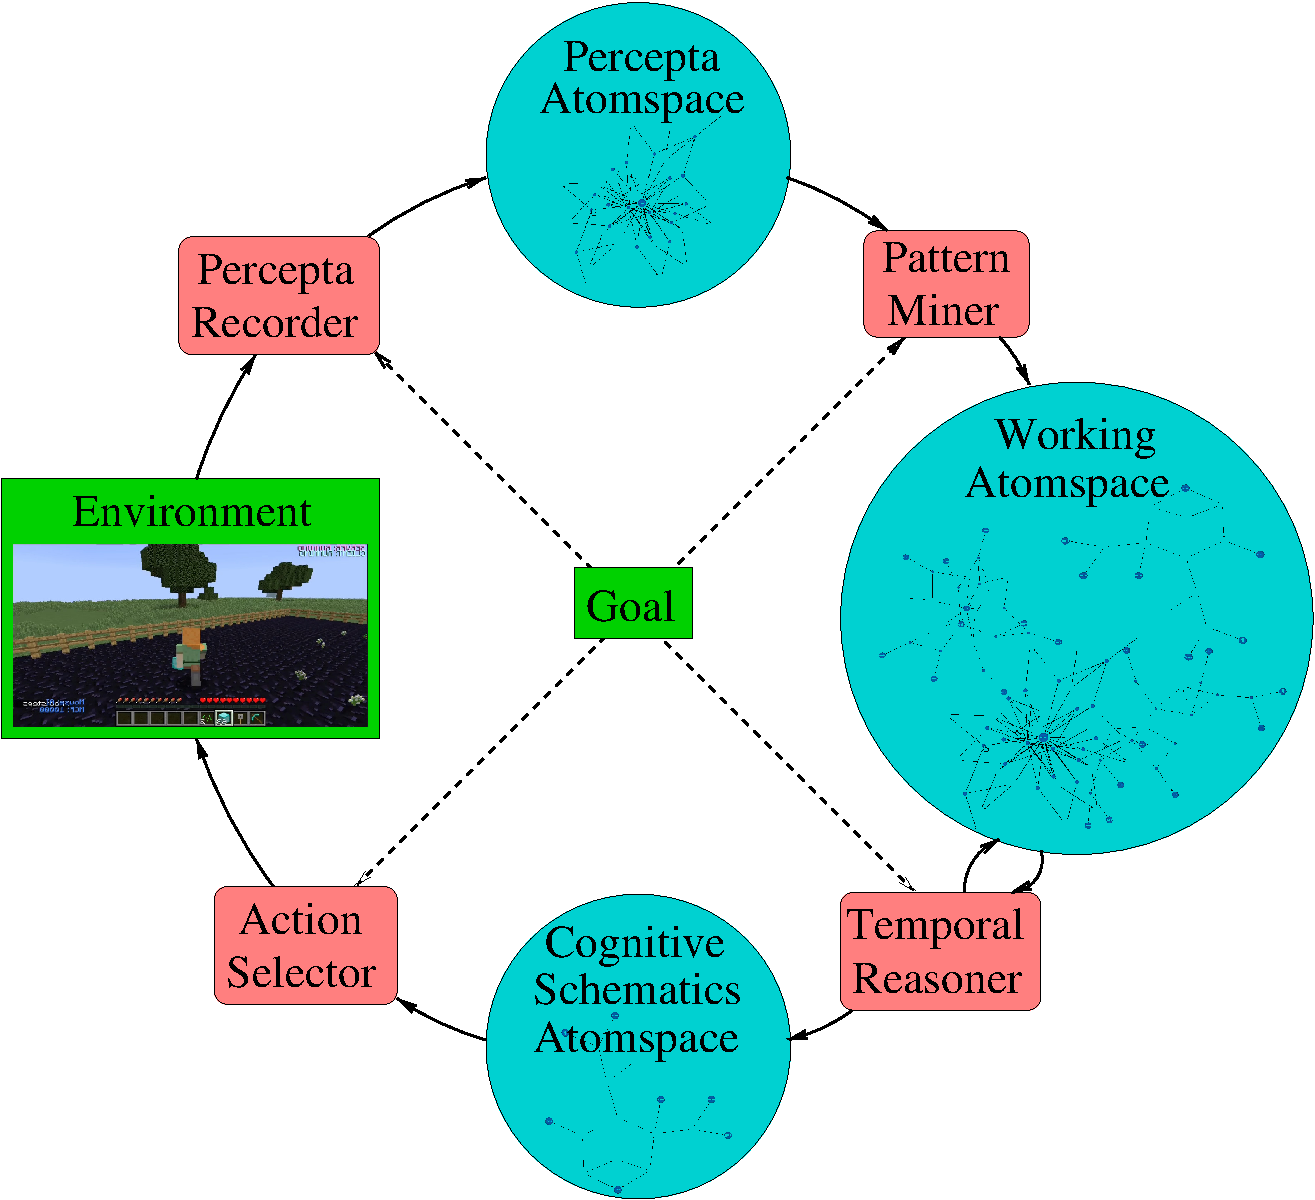
\includegraphics[width=1\textwidth]{pictures/rocca-chart-v0.6.pdf}

To experiment with temporal and procedural reasoning in the context of
embodied virtual agents in unknown environments we have implemented a
project called ROCCA, which stands for \emph{Rational OpenCog
Controlled Agent}.  ROCCA essentially acts as an interface between
virtual environments such as Malmo \cite{TODO} or OpenAI Gym
\cite{TODO} and OpenCog.  It provides an Observation-Planning-Action
control loop as well as various launchers to run OpenCog processes
such as PLN reasoning, pattern mining, etc.
%% During the life of the
%% agent control and learning phases are alternated to simulate a form of
%% online learning.
Provided a top goal, such as maximizing a reward, ROCCA orchestrates
the necessary learning and the planning to fulfill that goal.
%% somewhat like a reinforcement learning agent.
One may possibly see ROCCA as a reinforcement learning agent with the
particularity that learning and planning are, at least in principle,
entire done via reasoning.  In that respect it is similar in spirit to
OpenNARS for Applications (ONA) \cite{TODO} but uses PLN as its core
reasoning logic rather than NAL \cite{TODO}.
%% Where it differs from a typical
%% reinforcement learning agent in that both learning and planning are,

ROCCA is composed of two main processes, one for real-time agent
control and another one for non-reactive background learning.  In
principle these two processes could happen in parallel, though as of
right now they occur as distinct alternating phases.

\subsection{Control Phase}
The control phase is composed of control cycles, each decomposed into
Observation, Planning and Acting steps, more precisely
\begin{enumerate}
\item Observation step:
  \begin{enumerate}
  \item receives and timestamps observations from the environment,
  \item stores the timestamped observations in the atomspace.
  \end{enumerate}
\item Planning step:
  \begin{enumerate}
  \item selects the goal for that iteration,
  \item finds plans fulfilling that goal,
  \item given these plans, deduces a probabilistic distribution of
    actions,
  \item selects the next action according to the deduced probabilistic
    distribution.
  \end{enumerate}
\item Acting step:
  \begin{enumerate}
  \item timestamps and stores in the atomspace the selected action,
  \item runs the selected action and by that updates the environment,
  \item receives the reward from the environment,
  \item timestamps and stores the reward in the atomspace.
  \end{enumerate}
\end{enumerate}

None of these steps are difficult to carry with the exception of
deducing a probabilistic distribution of actions.  For that we use a
variation of Solomonoff induction described in \cite{TODO} which is
especially suited for plans described by conditional second order
distributions, in other words $\TPredImpl$ links.  More specifically
plans are $\TPredImpl$ links of the form
$$C \land A \lpreimp{T} G$$
called \emph{Cognitive Schematics}.  Which can be read as \emph{``in some
context $C$, if some action (elementary or composite) $A$ is executed,
then after $T$ time units, the goal $G$ is likely to be fulfilled''}.
The degree of expected fulfillment is specified by the truth value of
the $\TPredImpl$ link, not indicated in that notational format but
present in the extended Atomese format.  The difficulty then comes
down to discovering cognitive schematics that are as informative and
applicable as possible.

\subsection{Learning Phase}
As hinted above, the ultimate goal of the learning phase is to
discover maximally useful cognitive schematics, and by useful it is
specifically meant that they are as predictive and cover as many cases
as possible.

TODO: pattern mining and reasoning.

\section{Experiment with Simple Minecraft Environment}

In this experiment we built a minecraft environment using Malmo, which is a platform for Artificial Intelligence experimentation and research built on top of Minecraft. The demo environment consists of a small house with a locked door, diamonds inside and a key to get into the house. The agent, initially located outside of the house, can perform different actions like getting a key, opening a door of the house and collecting the diamonds in order to achieve a reward. \par
The aim of this experiment is to make the ROCCA agent learn from the actions and perceptions in the minecraft environment and do efficient planning so as to be able to collect as many diamonds as possible and accumulate reward. The ROCCA agent will be able to perform a series of possible actions with a goal of achieving a reward and learns from them by applying PLN (Probabilistic Logic Networks) and Pattern Miner, which can be seen as a specialized form of PLN reasoning. The Planning, the discovery of cognitive schematics, is also handled by PLN and its temporal reasoning rule base.

\begin{figure}[htbp]
\centerline{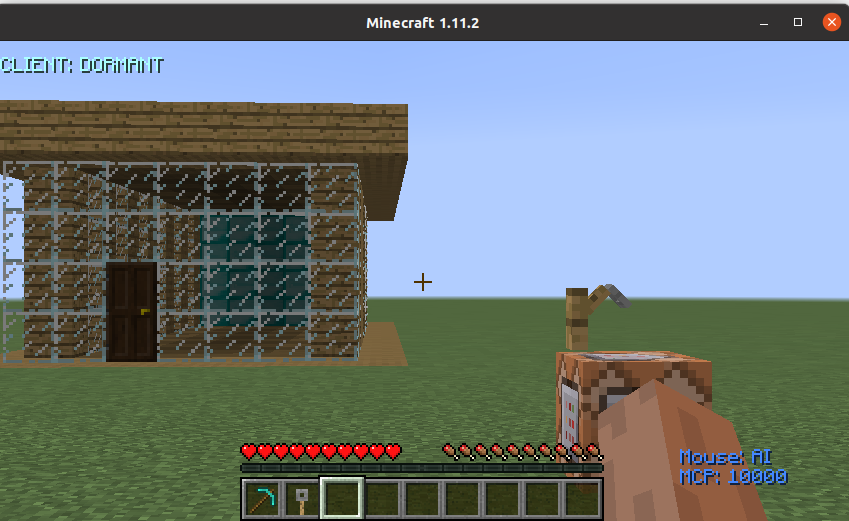
\includegraphics[scale=.2]{pictures/simple_demo.png}}
\caption{Simple Minecraft demo with a house and a key.}
\label{fig}
\end{figure}

There are lists of allowed actions provided by minecraft that an agent can perform like moving, turning, picking etc.. but due to the limited processing capacity we have to handle the observations from each action and to reduce complexity, we proposed to have an abstract action and perception where unnecessary details have been omitted. With that we generate three abstract actions namely go-to-key, go-to-house, go-to-diamonds where each of them contains a series of actions and returns an abstract perception about where the agent is (inside house, outside house, next to closed door etc..), about its inventory (has key, diamond pickaxe etc..) and the reward of completing a given action. \par
We perform various experiments tuning different parameters. A typical experiment has two iterations of the learning-training process with a duration of fifty iterations for each training. In the first cycle the agent will not have prior knowledge hence no learning will take place. The agent pursues the environment and builds its knowledge base by trying a combination of fifty randomly weighted actions. At the end of the first cycle the agent will have enough background knowledge to apply Pattern miner and PLN temporal reasoning. Hence, during the second cycle, the agent will be able to learn and plan the desired cognitive schematics which leads to a positive goal of getting a reward.\\
The ROCCA agent is able to learn the following cognitive schematics with higher strength.

$$\textit{outside}(\textit{self}, \textit{house}) \land \ldo{\textit{go\_to}(\textit{key})} \lpreimp{1} \textit{hold}(\textit{self}, \textit{key})$$
$$\textit{hold}(\textit{self}, \textit{key}) \land \ldo{\textit{go\_to}(\textit{house})} \lpreimp{1} \textit{inside}(\textit{self}, \textit{house})$$
$$\textit{inside}(\textit{self}, \textit{house}) \land \ldo{\textit{go\_to}(\textit{diamond})} \lpreimp{1} \textit{reward}(1)$$

In this experiment, we measure the agent's performance by the cognitive schematics learned and accumulated rewards achieved. The ROCAA agent is successful in learning the required cognitive schematics which leads the agent to collect more rewards in the second cycle. However, these findings with a simple minecraft environment with only few actions might not tell the overall performance of ROCCA. As a future work, further extensive experiments are needed to conclude the performance achieved.

\section{Conclusion}

TODO: implement more temporal and procedural rules, support temporal
intervals, behavior trees, introduce Temporal Truth Value.  Integrate
Event Calculus.

%
% ---- Bibliography ----
%
\bibliographystyle{splncs04} \bibliography{TPRC}

\end{document}
